% !TEX encoding = UTF-8 Unicode
%----------------------------------------------------------------------------
\chapter{Integration to \eiq}
%----------------------------------------------------------------------------
\label{chap:integration}

%TODO kb. 16-27 oldal

In this chapter the design and integration challenges are discussed in details. The implemented local search-based algorithm is from the paper \cite{DBLP:journals/sosym/VarroDWS15}. The main advantage of this algorithm is its adaptive model sensitive approach for calculating search plans. It means that the properties of the instance model, on which the search plan calculation is executed, are considered. In this work we only introduce the main differences and key ideas that were required for a successful implementation and integration.

%----------------------------------------------------------------------------
\section{Details of the adapted algorithm}
%----------------------------------------------------------------------------
\label{sec:details}


%TODO kb. 5-10 oldal

The published paper~\cite{DBLP:journals/sosym/VarroDWS15}, which served as the basis of our implementation, is about pattern matching over EMF models. However, it did not include any programming source code, only pseudo code. For this reason, we adapted it to be executable on a JVM, and to also fit into the internal design of \eiq. The current section introduces the concept of search plan, and the outline of the search plan calculation algorithm, along with an illustration of its execution on our running example. For a fully comprehensive description please refer to the article cited above.

%As we mentioned at the beginning of \autoref{chap:integration}, including every detail about the implemented search algorithm is far beyond the scope of this thesis, but the basic idea of search plan calculation is introduced in \autoref{sec:localsearch} for the better comprehensibility of our work.  

\subsection{Search plan}
\label{sec:localsearch}
	 
	 
A search plan, in our case, means an ordered list of constraints of the pattern definition. As it was discussed in \autoref{sec:pattern-matching-workflow}, the list of executable environment specific search steps are obtained by compiling the search plan. This compilation is simply a mapping between constrains and search steps, which only depends on the properties of the target modeling environment. For this reason, in the following we are only concerned about the search plan calculation. In the following we will refer to elements of the search plan as \emph{search operations}, and we will represent them with the corresponding constraint from the query definition.


In order to clarify the purpose of the search plan, we define the concepts of \emph{free variables} and \emph{bound variables}. They can be interpreted as follows: if the search execution of the search plan was halted at a given point, which variables would already be assigned to a model element, and which variables would not have values yet. Variables without associated values are called \emph{free variables} (\texttt{F}), and variables with assigned values are referred as \emph{bound variables} (\texttt{B}). 

The \emph{pattern adornment} denotes the initial binding state of the parameter variables of a pattern at the beginning of the pattern matching, in other words describes witch parameter variables have initial values. The purpose of the search plan is to guide the search execution in a way that by reaching the end of the search plan each variable should already be bound.



The search operations can be categorized according to the binding state of the variables affected by the corresponding constraint. Two basic categories of search operations are \emph{extend}, and \emph{check}. A \emph{check operation} verifies whether a variable substitution is in compliance with a constraint included in the pattern. This means that in case of a check, every variable of the operation is bound by the time of its execution. On the other hand, an \emph{extend operation} has a list of substitution values for a variable, where these values are selected based on the corresponding constraint. During the search, all the elements in this list are to be substituted in order to find all matches in the model.

As a corollary of the definitions of check and extend operations, we can say that the position of the operation in the search plan decides to which category it belongs. However, there are some disallowed extend cases, which require a significant computational capacity during search execution, thus they are to be avoided in a search plan. For instance, negative pattern calls should always be check operations.


%For instance, if base index is not built over a model, we inverse navigation along references without inverse navigability support would require an iteration over every object in the domain of the type of the source element of the reference.



In the example, to find all occurrences in a given ASG of the code smell described by \catchproblem, the initial adornment should be \texttt{FF}, which means both \texttt{cBlock} and \texttt{insOf} parameters are unbound at the start of the pattern matching process. A possible search plan for the \catchproblem pattern is included in \autoref{tab:catchproblemOriginal}.

\begin{table}[h]
	\centering
	\begin{tabular}{c|l|c|c}
		\hline
		& \multicolumn{1}{|c|}{Operation} & Type & Bound variables \\ \hline
		1: & \texttt{Indentifier(varRef)} & extend & $\{ \}$\\
		2: & \texttt{Unary.operand(insOf, varRef)} & extend & $\{ \texttt{varRef} \}$\\
		3: & \texttt{InstanceOf(insOf)} & check & $\{ \texttt{varRef, insOf} \}$\\
		4: & \handlervar$(\texttt{cBlock, varRef})$ & extend & $ \{\texttt{varRef, insOf}\} $ \\
		5: & \texttt{cBlock} is a \texttt{Handler(cBlock)} & check & $ \{\texttt{varRef, insOf, cBlock}\} $ \\
	\end{tabular}
	\caption{Search plan for pattern \catchproblem}
	\label{tab:catchproblemOriginal}
\end{table}

For there are no bound variables initially, the search plan starts with an extend operation. In this case it is an enumeration of instances of type \texttt{Identifier}. In the next step, by an \emph{inverse navigation} from the bound \texttt{varRef} variable, along the \texttt{operand} relation possible elements for \texttt{insOf} are collected. When using the \eiq Base Index over a model, inverse navigation along edges are possible, even if the reference has no inverse in the metamodel. The third step is a check operation, which makes sure whether the value of \texttt{insOf} is of type \texttt{InstanceOf}. The fourth operation is an extend, for it binds the \texttt{cBlock} variable by calling the pattern \handlervar with an adornment \texttt{FB}. As the result of the pattern call, each possible \texttt{Handler} block is collected for the value of \texttt{varRef}. In the final step of the search plan, the substituted value for \texttt{cBlock} is verified to be of type \texttt{Handler}. Note, that after the last search operation all variables are bound.

The search plan for the referred \handlervar pattern with initial pattern adornment \texttt{FB} is shown in \autoref{tab:handlervarOriginal}. 
However, we do not introduce the execution steps, because it is very similar to the steps of the search plan introduced for the \catchproblem pattern, except its initial pattern adornment is \texttt{BF}, which means that \texttt{cBlock} already has an assigned value.

\begin{table}[h]
	\centering
	\begin{tabular}{c|l|c|c}
		\hline
		& \multicolumn{1}{|c|}{Operation} & Type & Bound variables \\ \hline
		1: & \texttt{Handler(cBlock)} & check & $\{ \texttt{cBlock} \}$\\
		2: & \texttt{Handler.parameter(cBlock, param)} & extend & $\{ \texttt{cBlock} \}$\\
		3: & \texttt{Identifier.refersTo(variable, param)} & extend & $\{ \texttt{cBlock, param} \}$\\
		4: & \texttt{Identifier(variable)}  & check & $\{ \texttt{cBlock, param, variable} \}$\\
	\end{tabular}
	\caption{Search plan for pattern \handlervar}
	\label{tab:handlervarOriginal}
\end{table}


To demonstrate the importance of flattening and normalization, we include a possible search plan for the pattern from \autoref{lst:catch_flat_normalized} in \autoref{tab:catch_flat_normalized}. As we previously discussed in \autoref{sec:pattern-matching-workflow}, the flattened and normalized patterns have the same semantics as the original. However, the search plan for the normalized pattern is \emph{simpler} than the two original search plans together, where by simple we mean it has less steps of the same operation type than the search plans calculated for the original descriptions.

%TODO introduce alternative search plans?

\begin{table}[h]
	\centering
	\begin{tabular}{c|l|c|c}
		\hline
		& \multicolumn{1}{|c|}{Operation} & Type & Bound variables \\ \hline
		1: & \texttt{Identifier(varRef)} & extend & $\{ \}$ \\
		2: & \texttt{Unary.operand(insOf, varRef)} & extend & $\{ \texttt{varRef} \}$\\
		3: & \texttt{InstanceOf(insOf)} & check & $\{ \texttt{insOf, varRef} \}$\\
		4: & \texttt{Identifier.refersTo(varRef, param)} & extend & $\{ \texttt{insOf, varRef} \}$\\
		5: & \texttt{Handler.parameter(cBlock, param)}  & extend & $\{ \texttt{insOf, varRef, param} \}$\\
		6: & \texttt{Handler(cBlock)}  & check & $ \stackedlines{ \texttt{\{insOf, varRef,}}{\texttt{param, cBlock}\}} $ \\
		
	\end{tabular}
	\caption{Search plan for the flattened and normalized pattern}
	\label{tab:catch_flat_normalized}
\end{table}




\subsection{Search plan calculation}

To find the ordering of the constraints that yields an efficient search plan is a non-trivial task. To estimate the time needed to execute the matching, we can assign \emph{costs} to search operations, and from the individual costs of the operations we can derive the cost for the complete search plan. \emph{Cheap} search plans are desired, for it means that the search can finish faster according to our cost estimation.

In addition to \autoref{tab:catch_flat_normalized}, the search plan listed in \autoref{tab:catch_flat_normalized_from_debugger} can also be used to find matches for the \catchproblem pattern, they only differ in the order of operations. It is model-dependent, which provides faster execution.

\begin{table}[h]
	\centering
	\begin{tabular}{c|l|c|c}
		\hline
		& \multicolumn{1}{|c|}{Operation} & Type & Bound variables \\ \hline
		1: & \texttt{Handler(cBlock)} & extend & $\{ \}$\\
		2: & \texttt{Handler.parameter(cBlock,param)} & extend & $\{ \texttt{cBlock} \}$\\
		3: & \texttt{Identifier.refersTo(varRef, param)} & extend & $\{ \texttt{cBlock, param} \}$\\
		4: & \texttt{Identifier(varRef)} & check & $\{ \texttt{cBlock, param, varRef} \}$\\
		5: & \texttt{Unary.operand(insOf, varRef)}  & extend & $\{ \texttt{cBlock, param, varRef} \}$\\
		6: & \texttt{InstanceOf(insOf)}  & check & $ \stackedlines{ \texttt{\{insOf, varRef,}}{\texttt{param, cBlock}\}} $ \\
		
	\end{tabular}
	\caption{An alternative search plan for \catchproblem}
	\label{tab:catch_flat_normalized_from_debugger}
\end{table}

\subsubsection{Calculating the cost of a search plan}

The search plan calculation algorithm described in~\cite{DBLP:journals/sosym/VarroDWS15} proposes a method to calculate \emph{operation weight} to encode the estimated costs of the operations and search plans. Our current implementation of the algorithm applies the proposed solution with minor modifications.

The main idea is to take every constraint form the pattern, and generate search operations with all possible and allowed variable binding combinations. This means, for every constraint it generates $2^a$ search operations, where $a$ is the number of variables affected by the constraint. This could results in several search operation objects, however, typically constraints have 1 or 2 variables, and for pattern call constraint, we only allow \texttt{BB\ldots B} adornments. We can say that in practical applications, the result search operation set will not reach extreme sizes typically. In the final search plan \emph{each constraint will be represented by exactly one search operation}, and the unused ones will be discarded.
 
Along with the creation of search operations, an estimated number of potential substitutions values is calculated, which the executor has to check each time, when it is executed. This number is then used as its \emph{weight} or \emph{cost}. This means that check operations have a weight of 1, for they only verify whether the current substitutions satisfy a constraint. 

For extend operations, we distinguish several cases. If the operation affects only one variable, which is in case of \eiq means a type constraint, then the cost of the operation is the cardinality of the type required by the constraint. In case of operations enforcing an IQPL path expression, which define that two model elements are connected by an \texttt{EReference} instance, there can be three cases according to the binding state of the of the affected variables:

\begin{itemize}
	\item \texttt{FF}: this operation adornment is disallowed.
	\item \texttt{BF}: in this case the cost is estimated with the \emph{average branching factor}, given by the formula $\textit{weight} = \dfrac{\textit{cardinality of source class}}{\textit{number of links}}$.
	\item \texttt{FB}: similarly to the previous case, the average branching factor is calculated by \\$\textit{weight} = \dfrac{\textit{cardinality of target class}}{\textit{number of links}}$.
\end{itemize}

Every other type of constraint, that is not flattened or normalized (\texttt{count find}, \texttt{neg find}, and inequality) are not allowed as extend operations, for they would typically require unmanageable search times. Positive pattern calls are at the moment always flattened.
%, which often can even be infinite, \eg for inequality.

The cited article distinguishes other constraint types as well, such as ternary constraints for ordered references, but in \eiq there is no support to directly input such constraints yet.

From the $w_{o_{k}}$ costs for each $o_k$ operation, where $k$ represents the position in the search plan, the total cost $C_n$ of a search plan containing $n$ search operations is calculated with the following recursive formula:

$$ C_n = \sum_{i=1}^{n} \prod_{j=1}^{i} w_j = C_{n-1} + w_{o_{1}} \cdot w_{o_{2}} \cdots \cdot w_{o_{n}}. $$
\label{sec:cost}

\subsubsection{Dynamic programming based search calculation}

With the above definition of search plan cost, a dynamic programming based approach is used to create search plans that are cheap in this sense. The algorithm outline is as follows:

\begin{enumerate}
	\item Initialize a table with dimensions $d \times (f+1)$, where $d$ is an input parameter of the algorithm. We call it \emph{drop threshold}, because it influences which search plans are considered too expensive during the planning process, and thus ignored in later steps. The $f$ symbolizes is the \emph{number of free variables} in the initial adornment of the pattern. Each column symbolizes the number of free variables, and each cell represents a search plan. Column indices go from $f$ to $0$.
	\item Starting from the $f$th column, we begin filling out the table using the rules below:
		\begin{itemize}
			\item Based on a previous search plan, we pick an \emph{applicable} extend operation, which means every variable affected by the operation and marked with \texttt{B} in its adornment is bound by the end of the previous search plan, and every variable marked with \texttt{F} in the operation adornment is free at the end of the selected, preceding search plan. When done, we append it to the search plan. In case we are filling out the $f$th column, and there is no preceding, then create a new one instead.
			\item Append all applicable check operations to the search plan, then calculate a new cost using the recursive formula.
			\item Insert search plans calculated this way in an increasing cost order to the table, and simply drop search plans that do not fit. The number of search plans in a column is determined by the parameter $d$.
		\end{itemize}
	\item Select the plan that is in the intersection of the first row and $0$th column, because has the lowest cost, and yields \texttt{BB\ldots B} variable binding after its final step.
\end{enumerate}


Two steps of the running algorithm on the model depicted in \autoref{fig:example-instancemodel-handdrawn}  is demonstrated in \autoref{fig:plan-calculation-example} by filling up the columns 4, 3 and 2 of the table of search plans. The $d$ parameter is set to $2$.

\begin{figure}[!htp]
	\centering
	\includegraphics[width=\textwidth]{figures/pdfs/plan-calculation.pdf}
	\caption{Table of search plans}
	\label{fig:plan-calculation-example}
\end{figure}

Initially column 4 contains only one entry, which is a search plan with an empty list of operations, total cost of 0, and an empty set of bound variables. Based on the variable binding, the applicable constraints are \texttt{Handler(cBlock)}, \texttt{Identifier(varRef)}, and \texttt{InstanceOf(insOf)}, all with adornment \texttt{F}. 

In the first step, the cost of the search plans containing only one of them is calculated. Using the recursive cost formula, it gives the cost of the operation plus the cost of the preceding search plan, which is in this case 0. Based on the instance model the costs are 1 for \texttt{Handler(cBlock)}, 2 for  \texttt{Identifier(varRef)}, and 1 for \texttt{InstanceOf(insOf)}. The search plans are then inserted into column 3 in increasing cost order. We chose $d = 2$, so the third search plan is discarded, which means it is not stored in the table, thus not used as the basis of latter search plans.

In the second illustrated step, the same considerations are applied. First, the applicable search operations are collected for the search plans: \texttt{Handler.parameter(cBlock,param)} with adornment \texttt{BF} is for the plan in column 3, row 1, and \texttt{Unary.operand(insOf, varRef)} with adornment \texttt{BF} for the plan in column 3, row 2. Other operations are currently not available, neither extend operations, nor check operations, so only one new plan is derived for each of them.  We can estimate the cost for \texttt{Handler.parameter(cBlock,param)} to $\dfrac{1}{1} = 1$, because our simple example model contains only 1 \texttt{Handler} element, that has only one \texttt{parameter} link. Similarly for \texttt{Unary.operand(insOf, varRef)} the cost is also 1. In both cases the costs of the new search plans will add up to $1 + 1 * 1 = 2$, using the recursive cost calculation formula again.

We do not introduce the complete run, but the paper~\cite{DBLP:journals/sosym/VarroDWS15}, from which we adapted the algorithm, contains a complete running example on the process of calculating the search plan.

The complexity of the implemented algorithm is $\mathcal{O}(|V|^2 \cdot |O|^2)$, where $V$ denotes the set variables, while $O$ marks the set of constraints included in the pattern. The parameter $d$ simplifies the calculation, because the plans that are more likely to have too high costs are discarded immediately, and not taken into account in later steps. However, if this value is chosen to be too small, the algorithm will execute similarly to a \emph{greedy algorithm}. According to our experiences, choosing $d=4$ is a reasonable setting for practical applications.





%----------------------------------------------------------------------------
\section{Implementation details}
%----------------------------------------------------------------------------
\label{sec:implementation}

This section summarizes the main design decisions that were followed during the implementation.
In \autoref{sec:matcher-api} the common matcher interface for both the local search and the Rete pattern matcher introduced. Then in \autoref{sec:flattening} the iterative flattener algorithm implemented for the local search planner is outlined. In \autoref{sec:lsdebugger} we describe the capabilities of the Local Search Debugger component, that can help developers to optimize the patterns.


\subsection{Common matcher API}
\label{sec:matcher-api}
In terms of development of \eiq, one of the biggest recurring questions is to decide for which extent we are supposed to provide a generic solution to a problem, and to which extent we should give a specialized solution. Before answering this question, several aspects will be considered, such as modularity, reusability and backward compatibility. 

%They can heavily influence the opinion of the users

When we decided to provide matchers that use the local search-based pattern matching algorithm for finding matches, there was already an existing Rete algorithm-based matcher implementation. To prevent breaking the API and causing backward incompatibility, the functions of the \texttt{RetePatternMatcher} were pulled up to an interface called \texttt{IQueryResultProvider}. For the new algorithm, a new class \texttt{LocalSearchResultProvider} was created that implements the (now common) \texttt{IQueryResultProvider} interface. This way users who already worked with a \texttt{RetePatternMatcher} can still do so, while users of the new API are advised to access a result provider via the \texttt{IQueryResultProvider} interface. \autoref{fig:resultprovider-class} shows the class diagram of the current solution.

\autoref{fig:resultprovider-class} illustrates the classes that are associated with the new \texttt{LocalSearchResultProvider}. The provider has a \texttt{LocalSearchPlanner} and a \texttt{LocalSearchMatcher}. The former is responsible for the search plan calculation, while the latter contains the search execution code. The planner has dedicated components for each process depicted in \autoref{fig:workflow}: \texttt{PQueryFlattener}, \texttt{PQueryNormalizer}, \texttt{LocalSearchPlannerStrategy}, and \texttt{POperationCompiler}, respectively.

\begin{figure}[!htp]
	\centering
	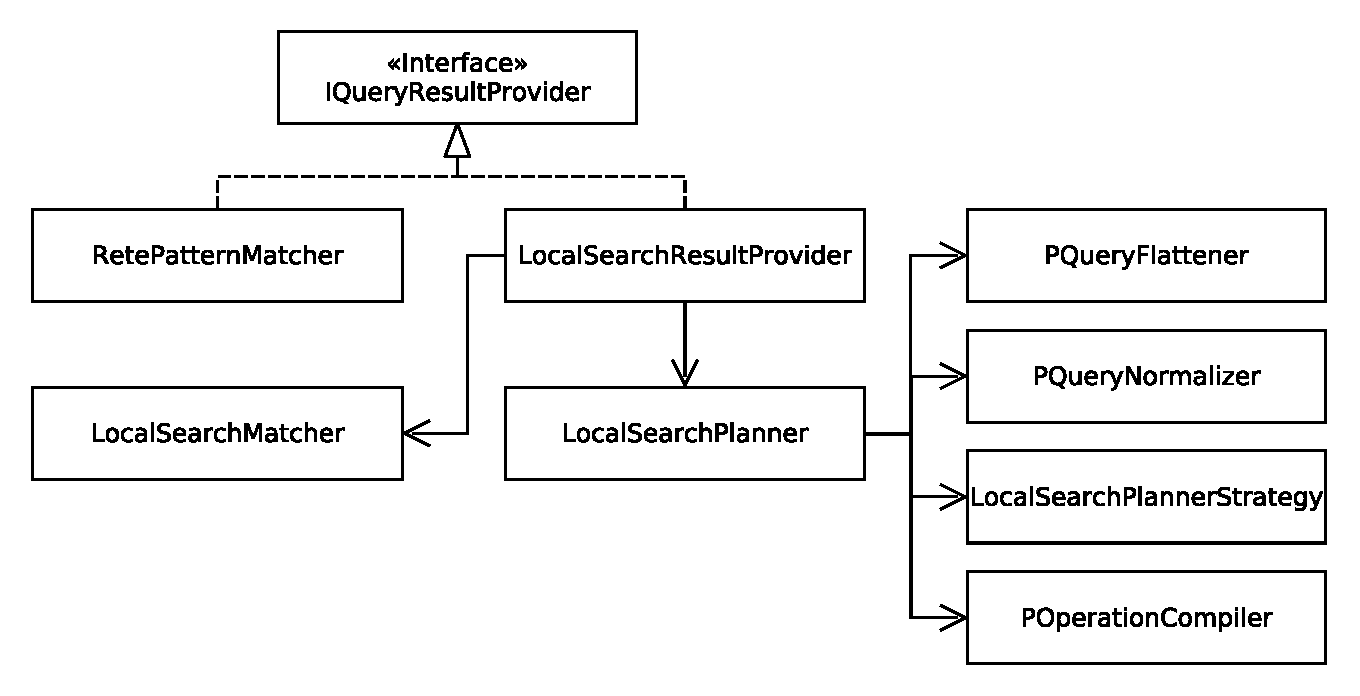
\includegraphics[width=\textwidth]{figures/pdfs/matcher-class-diagram.pdf}
	\caption{The internal structure of the new result provider}
	\label{fig:resultprovider-class}
\end{figure}

We reused the normalizer from the Rete algorithm. The other three components, which also realize steps of the search plan calculation workflow, are created with respect to modularization. Each provide a functionality that may be later replaced with a new implementation. This is especially true for the \texttt{LocalSearchPlannerStrategy}. It holds the business logic for the search plan calculation, so if an alternative version is to be created, only this component should be replaced or changed. 



\subsection{Flattening}
\label{sec:flattening}
 
 The flattening is a novel feature in the \eiq framework. It is not needed by the Rete pattern matcher, but in case of local search-based pattern matching it supports cheaper search plan calculation. Pseudo code of the core algorithm used for flattening is shown in Algorithm~\autoref{alg:flattening}.
 
 
 
 \begin{algorithm}[H]
 	\label{alg:flattening}
 	\caption{Flattening}
 	
 	
 	\SetKwInOut{Input}{input}
 	\SetKwInOut{Output}{output}
 	
 	\SetKwData{PreStack}{preStack}
 	\SetKwData{PostStack}{postStack}
 	\SetKwData{PatternDescription}{patternDescription}
 	\SetKwData{Item}{item}
 	\SetKwData{FlatQueries}{flatBodies}
	\SetKwData{CalledPattern}{calledPattern}

 	
 	
  	\SetKwFunction{Push}{push}
  	\SetKwFunction{Pop}{pop}
  	\SetKwFunction{CopyCalledIntoCaller}{copyCalledIntoCaller}
  	
  
  	\Input{A pattern \PatternDescription}
  	\Output{Semantically equivalent, flattened pattern}
  	
  	\BlankLine
 	
 	\PreStack $ \leftarrow \emptyset $;
 	\PostStack $ \leftarrow \emptyset $; \label{line:init}
 	
 	\PreStack.\Push\functionCall{\PatternDescription}; \label{line:start}

	\While{ \PreStack not empty }{ \label{line:pre-begin}
		\Item = \PreStack.\Pop\functionCall{};
		
		\PostStack.\Push\functionCall{\Item}; \tcp*[f]{Schedule for flattening}
							
		\For{\CalledPattern $\in$ set of patterns called by \Item}{
			\If{\CalledPattern needs flattening} {
				\PreStack.\Push\functionCall{\CalledPattern};  	\tcp*[f]{Fill up \PreStack  \hspace{40pt}}
			}
		}
	}\label{line:pre-end}
	
	\While{ \PostStack not empty }{ \label{line:post-begin}
		\Item = \PostStack.\Pop\functionCall{}; \tcp*[f]{Take out for flattening} \label{line:item-pop}
		
		\Item.\CopyCalledIntoCaller\functionCall{};
	}\label{line:post-end}
	
 \end{algorithm}



In \autoref{line:init} two empty stacks are initialized: \texttt{preStack} holds the patterns that are encountered during the traversal of the call tree, while \texttt{postStack} holds patterns that need to be flattened, and all the referred patterns are flat. In \autoref{line:start} the parameter pattern is scheduled for flattening. To flatten all calls, a \emph{preorder depth-first traversal} is done on the pattern call tree between \autoref{line:pre-begin} and \autoref{line:pre-end}. This collects all calls that are necessary to be flattened at some point. This cycle leaves patterns untouched, only inserts them to the \texttt{preStack} by the time they are encountered during the traversal of the call tree.

From \autoref{line:post-begin} to line \autoref{line:post-end} postorder actions are carried out. At this point we know, that the \texttt{item} in \autoref{line:item-pop} is a pattern that may refer only to flattened patterns, or to patterns that need no flattening. For this reason, the only remaining task is to copy the called patterns into the caller. The function \texttt{copyCalledIntoCaller} leaves the pattern untouched, in case it needs no flattening, in other cases it merges the called pattern constraints and variables to the caller. The reason for this can be the pattern contains no call, or some predicate tells that the pattern should not be flattened.

This algorithm can be used efficiently to flatten pattern calls. However, \eiq has language constructs, for which flattening cannot be applied, namely \texttt{neg find}, \texttt{count find}, and \emph{binary transitive closure}. In these cases the matching should be done by calling matchers for the referenced queries.

A limitation of the current implementation is the lack of support for recursive queries. This algorithm would end up in an infinite loop, if a recursive query was its input. For this reason, in the current implementation the planner first checks for recursion. If the pattern is not recursive, flattener can proceed, otherwise an exception is thrown.

\subsection{Debugger tooling}
\label{sec:lsdebugger}

This description of the Local Search Debugger tooling is from the paper~\cite{DBLP:conf/gg/BurUHV15}. The high-level, declarative nature of graph patterns sometimes results in hard to understand corner cases. In such cases simply looking at match results, as supported by the Query Explorer, does not provide enough details to locate the source of the problem. To support this use case, the development environment of \eiq has been extended with a \emph{Local Search Debugger} view that follows through the execution of a search plan created for a pattern over a model.

As constraints of graph patterns are often not evaluated in the order of their definitions, it is hard to see which constraints are already evaluated during search execution. On the other hand, the ordered search operations visualize the status of pattern matching, and can be traced back to the source pattern. The view can also be used for pattern matching execution optimization, similar to explain plans~\cite{oracle-enterprisemanager} used for optimizing SQL queries.

As \autoref{fig:lsdebugger} depicts a screenshot of the tool. Its view has four distinct parts to display information about as well as to control the execution. At the upper left corner (a) the search plan itself is shown, including the plans created for called patterns. Each line represents a search operation, and child nodes are operations of a called pattern. The current status of the execution is indicated with a set of icons: check marks are assigned to executed operations, question marks are assigned to operations not yet started, while the current operation is denoted with the 'Run' symbol. In this screenshot, the search plan contained in \autoref{tab:catch_flat_normalized_from_debugger} is displayed for the \catchproblem pattern. It is also extended with a final virtual search step called \emph{Match found}, which is only used to visualize the event of finding a match. The execution is halted after the execution of the first three extend operations, and the following check is ready for execution.


\begin{figure}[!htpb]
	\centering
	\includegraphics[width=\textwidth]{figures/ls-debugger-tooling}
	\caption{Local search debugger view}
	\label{fig:lsdebugger}
\end{figure}

In the bottom left corner (b) a set of tables is presented on different tabs summarizing the found matches. The tabs have the same name as the corresponding pattern, and the tables include the found matches of all patterns in different tables on different tabs, including both parameters and local variables. In \autoref{fig:lsdebugger}, currently variables \texttt{cBlock}, \texttt{param}, and \texttt{variable} are assigned a value, and \texttt{insOf} is \texttt{null}, which indicates that it is not bound to a value.

In the right side (c) of the view, a graph representation is provided for the currently evaluated (partial) match, showing the current substitutions for the pattern variables along with the relationships between them. The example screenshot depicts that there is an object of type \texttt{Handler} (bottom), which is linked to a \texttt{Parameter} instance (middle). The \texttt{Parameter} instance is further linked to an object of type \texttt{Identifier} (top). The presentation also contains the names and types of objects, and the names of relations.

Finally, to control the execution, (d) standard debugging operations are available~\cite{seifert2008debugging}. Breakpoints can be assigned to search operations either by selecting the operation and clicking on the bug icon, or by double clicking on an operation in the search plan. In addition, both step-by-step and continuous execution modes are available. The former is indicated with the \emph{step into}, the latter is with the \emph{continue halted execution} icon. To initiate the pattern matching process, the play button should be pressed after selecting the desired pattern in the Query Explorer.

This view complements the debugging capabilities of the Query Explorer, as the latter one is useful for identifying problematic cases by providing live feedback when the model changes, while the former visualizes the detailed execution of the search. The local search algorithm, in our experience, works similarly as a query developer reasons about a graph pattern, thus it eases the understanding of complex graph patterns.

%----------------------------------------------------------------------------
\section{Details of search execution}
%----------------------------------------------------------------------------
\label{sec:search-execution}

%Parallelization types: 'level0' and 'level1'
%Figures: visualize the parallelization types

The search execution relies on the search plan to find suitable substitutions for the variables of the pattern. In the following sections a sequential, and a parallel execution approach is introduced in \autoref{sec:sequential-search}, and in \autoref{sec:parallel-search}, respectively.

%TODO{write about environment specific search steps?}

\subsection{Sequential search}
\label{sec:sequential-search}


A generic structure for a search plan is depicted in \autoref{fig:sequential-searchplan}. If an operation is scheduled for th first execution, is \emph{initialized}, then \emph{executed}. A search execution should always start with the initialization of the first operation.


\begin{figure}[!htp]
	\centering
	\includegraphics[width=\textwidth]{figures/pdfs/sequential.pdf}
	\caption{Search plan as list of search operations}
	\label{fig:sequential-searchplan}
\end{figure}

For extend operations, the initialization means gathering all elements of a type, or enumerating model elements that are navigable from a reference of a given object. In general terms, it initializes a collection of potential substitutions for a variable. When executing the extend operation, there can be be two outcomes, which are \emph{success} or \emph{failure}. In case of success, the next value from the collection was successfully substituted into a variable. When execution fails, it indicates that there were no more potential substitutions available for the variable.

Initialization for check operations only means setting a boolean indicator \texttt{isExecuted} to \texttt{false}. When the check is executed, it sets \texttt{isExecuted} to true, and the substitutions of the affected variables are tested against the constraint that is assigned to the check operation. The result of the execution returns success, if the substituted values fulfill the requirements set by the constraint and the \texttt{isExecuted} flag was now set to \texttt{true}.

If the execution of an operation is successful, the executor may carry on to the next operation, otherwise it \emph{backtracks}. Upon backtracking, the previous operation is not initialized again, only executed. 

A match is found, when the last operation returns success. In this case, after storing the match, a backtrack is enforced on the last operation in order to find further matches, even though the operation returned success. Matching is finished, when the first operation returns failure.




A running example of the search is illustrated step-by-step in the followings. In this case the search is carried out on the example instance model captured in \autoref{fig:example-instancemodel-handdrawn}, and uses the search plan included in \autoref{tab:catch_flat_normalized}.


\autoref{fig:sst} displays the \emph{search space tree} for the example. Its nodes are symbolizing different states from the aspect of variable bindings. Each of them is represented by a table containing a header with the names of all variables in the pattern, and a single row containing the names of the substituted model elements. The minus sign ($-$) symbolizes that a variable is unbound. The parameter variables are in the left part of the tables, while the right part, which is separated by double vertical lines, holds the rest of the pattern variables.

%, where names are taken from \autoref{fig:example-instancemodel-handdrawn}. 
The directed edges are showing the possible transitions between the states by substituting a suitable value. There are no different states representing fully identical assignments to all variables.


\begin{figure}[!htp]
	\centering
	\includegraphics[width=\textwidth]{figures/pdfs/sst.pdf}
	\caption{Search space tree for search plan in \autoref{tab:catch_flat_normalized}}
	\label{fig:sst}
\end{figure}



In our running example, the search starts with unbound variables. In the first step, which is the execution of an extend operation, the executor collects all possible substitutions for \texttt{varRef} in a list, which is in this case \texttt{[file, e]}. Then, it substitutes \texttt{file}, which is the first element, to \texttt{varRef}, and \texttt{proceeds} to the next operation. In \autoref{fig:sst}, the newly substituted values are indicated with bold letters. However, the model does not contain any element of type \texttt{Unary} from which the element \texttt{file} would be navigable via the \texttt{operation} reference, and for this reason the executor \emph{backtracks}.

The next action is to substitute a new value to \texttt{varRef}, which is \texttt{e} with the type \texttt{Identifier}. Then again, the executor seeks for all \texttt{Unary} elements that has \texttt{e} as their \texttt{operand}. This case it gives a list of length 1, namely \texttt{[io]}. Then this only value is substituted to \texttt{insOf}. After substitution, it is made sure that its type is \texttt{InstanceOf} by the check operation, which is indicated by italic letters in the search space tree. Next, the elements of the \texttt{refersTo} relation is gathered, which is a list of containing the model element \texttt{e} of type \texttt{Parameter}, which is not to be confused with the \texttt{Identifier} already substituted to \texttt{varRef}. It is followed by collecting all objects from the model that can reach \texttt{e} via \texttt{parameter} reference. This case it is only the \texttt{hdl}, which is finally checked if it has the type \texttt{Handler}. This is also stands, so a match is found.

At this point the matching process is not over, for all other potential values gathered in extend operations should be tested, if they can form a match. For this reason, the execution backtracks until the last extend operation can pick a new value for substitution. However, this case every extend operations, including the first, have reached to the end of their list of substitution values. For this reason, after the backtracking is done, the pattern matching finishes.

%\todo{a more detailed introduction of search execution}

\subsection{Multi-threaded execution}
\label{sec:parallel-search}
%kb. 3-5 oldal

If a search plan contains at least one extend operation, it means that the executor will test each possible substitutions one-by-one. This provides an opportunity, to distribute the substitution tasks among multiple executors. We proposed a simple solution in which the search plan is forked at the first extend operation. These forks are assigned to separate executors running on different threads in order to harness the additional resources available in multi-core/Hyper-threading computers. The basic idea of the solution is illustrated in \autoref{fig:multithreaded-searchplan}

\begin{figure}[!htp]
	\centering
	\includegraphics[width=\textwidth]{figures/pdfs/parallel_level1.pdf}
	\caption{A possible parallelization of search plan execution}
	\label{fig:multithreaded-searchplan}
\end{figure}

We can assume that the first extend operation in the search plan is $o_i$ with the possible substitutions $e_1, e_2, \ldots, e_n$, and we also know that $e_p = e_q $ iff $p = q$, where $p,q \in [1,n]$. Then we can evenly distribute the values among $c$ processors by creating $c$ number of modified $o^k_i$ extend operations. These modified extends should have substitution values $e_{j_{k}+1}, e_{j_{k}+2}, \ldots, e_{j_{k+1}}$, where $j_k = (k-1) \cdot \left\lfloor\dfrac{n}{c}\right\rfloor $ for every $k = 1, 2, \ldots, c-1$, and $e_{j_{c}} = n$

Creating a copy of the operations marked as \textit{Rest of the search plan} in \autoref{fig:multithreaded-searchplan} is necessary, because the search operations are represented by stateful objects. Preserving a state is required for extend operations to maintain the internal collection of potential substitutions, and also required for check operations to handle backtracks with the \texttt{isExecuted} flag.

We can summarize our solution for parallelization in three steps:

\begin{enumerate}
	\item The task is to instantiate modified extend operations, marked with the $o^k_i$ in \autoref{fig:multithreaded-searchplan}, and distribute the candidate elements of the first extend among them.  This step also includes creating a copy from the rest of the search plan.
	
	\item Carry out sequential execution for each newly created search plan. Each executor should maintain its own result set, instead putting the matches in a shared collection. The latter option was also considered, but in order to avoid synchronization and blocking, we decided to merge the results in a separate step.
	
	\item Await all executors, then merge the results. The uniqueness of matches is automatically ensured by the fact that the modified extend operations work with disjoint lists of model elements, which is the result of the initial assumption of $e_p = e_q$ iff $p = q$, where $p,q \in [1,n]$.
\end{enumerate}

\subsection{Advantages and weaknesses}
\label{sec:advantages-weaknesses}

A huge advantage of the solution is the possibility to utilize all physical execution cores of the hardware. Based on \emph{Amdahl's law}, using a  CPU with $c$ cores, the time $t$ needed for the sequential \emph{the search execution} could drop to $(1-p) \cdot t + \dfrac{p}{c} \cdot t$, where $p \in [0,1]$ expresses the portion of the instructions that can run in parallel. If there was $ p \approx 1 $, it would yield $\dfrac{t}{c}$ for the new execution time.
This sounds promising, but the evaluation results in  \autoref{sec:performance-evaluation} and in \autoref{sec:performance-evaluation-tb} will show that the speedup in practice is not even close to this bound generally, which means a significant part of the instructions cannot run in parallel.

As a drawback, the solution has preparation overhead. This currently means the creation of the executor thread pool, the distribution of the model elements among executors, and the cloning of the rest of the search plan. Additionally, when creating sublist from the list of elements of the first extend operation, it is unknown how long will it take for the executor, until all matches that involve the element will be found. It may turn out soon that the value fails to fulfill even the constraint associated with the next check, but it is also possible that the substituted value is part of several matches, taking the executor long time to compute them all. 

